\chapter{Preliminary Results}

	\begin{itemize}
		\item For each long sound file
		\begin{itemize}
			\item find start and end points
			\item shift the sound pulse to beginning, middle and end
				to generate 3 sound files
		\end{itemize}
	\end{itemize}


\begin{figure}[h]
    \centering
    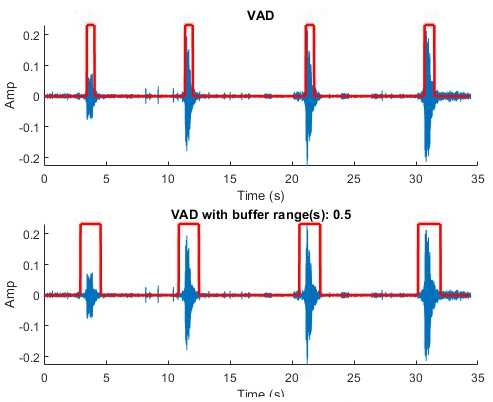
\includegraphics{aymen-audiosegment}
    \caption{Caption}
    \label{aymen-audiosegment}
\end{figure}

\begin{table}[h]
	\caption{Species used in preliminary experiments.}
    \label{tab:my_label}
    \centering
	\begin{tabular}{clc}
    \toprule
	\textbf{Number} & 
	\textbf{Species} &
	\textbf{Soundfile count} \\
	\midrule
	1 & \textit{Mareca penelope} & 1000 \\
	2 & \textit{Turdus migratorius} & 1000 \\
	3 & \textit{Alaudala cheleensis} & 1000 \\
	4 & \textit{Cinnyris asiaticus} &  1000 \\
	5 & \textit{Zenaida asiatica} & 1000 \\
	6 & \textit{Lanius collurio} & 1000 \\
	7 & \textit{Icterus icterus} & 1000 \\
	8 & \textit{Glaucidium cuculoides} & 1000 \\
	9 & \textit{Columba oenas} & 1000 \\
	10 & \textit{Terpsiphone viridis} & 1000 \\	
	\bottomrule
	\end{tabular}
\end{table}

\begin{figure}[h]
    \centering
    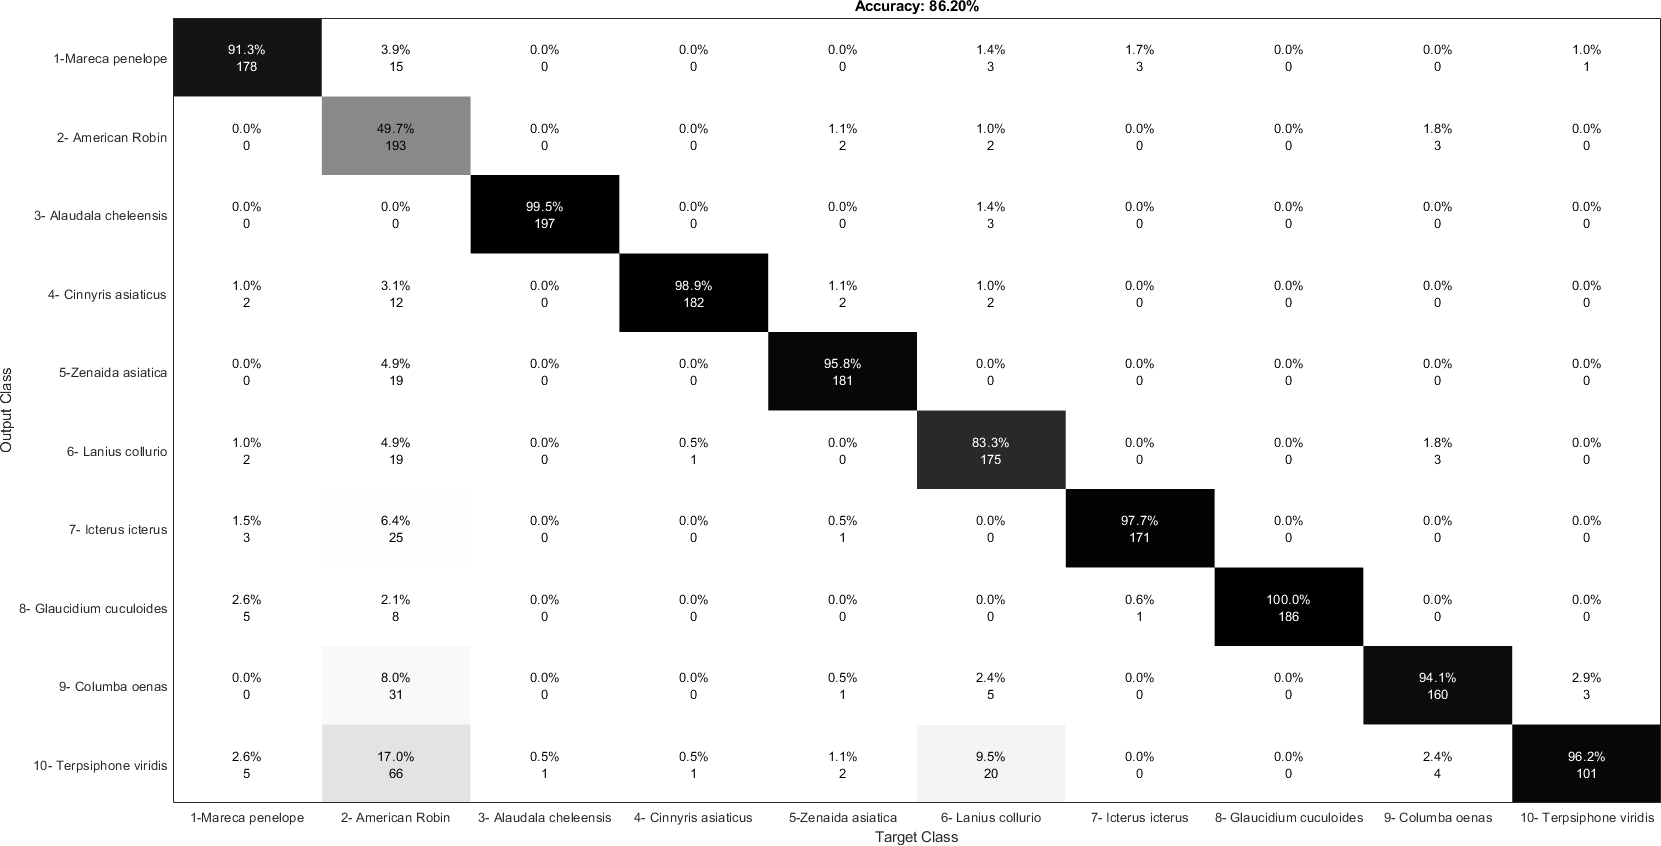
\includegraphics[width=\textwidth]{aymen-stft}
    \caption{STFT confusion matrix.}
    \label{aymen-stft}
\end{figure}


In this section, we propose a comprehensive qualitative evaluation of the proposed algorithms. Two platforms are targets:
\begin{itemize}
\item AMD FX-8350 at 4 GHz having eight cores, 8 MB cache and 32 GB DRAM supported by NVIDIA GTX 1080 Ti with 11 GB RAM
\item Raspberry Pi 3 containing quad-core ARM Cortex-A53 running at 1.20 GHz with 1 GB of RAM.
\end{itemize}

\noindent The reason for choosing different platforms is that the lightweight algorithms can differ in implementations depending on the use-case and deployment strategy
